%\VignetteIndexEntry{anchors}
%\VignetteDepends{anchors,MASS,rgenoud}
%\VignettePackage{anchors}
\documentclass{amsart}
\usepackage{natbib}

\newcommand{\code}[1]{{\texttt{#1}}}
\newcommand{\pkg}[1]{{\texttt{#1}}}
\newcommand{\Robject}[1]{{\texttt{#1}}}
\newcommand{\Rfunction}[1]{{\texttt{#1}}}
\newcommand{\Rpackage}[1]{{\texttt{#1}}}
\newcommand{\Rclass}[1]{{\textit{#1}}}
\newcommand{\Rmethod}[1]{{\textit{#1}}}
\newcommand{\Rfunarg}[1]{{\textit{#1}}}
\newcommand{\R}{{\normalfont\textsf{R}}{}}
\renewcommand{\S}{{\normalfont\textsf{S}}{}}
\newcommand{\AnchorsVer}{3.0-7}
\newcommand{\RVer}{2.8}
\newcommand{\AnchorsDate}{\today}
\newcommand{\ssubsection}[2]{%
  \subsection[#1]{\normalfont\scshape #1: {\tt #2}}}

\newcommand{\Ranchors}{{\texttt{anchors}}}
\setlength{\parskip}{1.2ex plus0.2ex minus0.2ex}

\usepackage{times}
\usepackage[all]{xy}        

%\usepackage{html}
\usepackage{url}
% \newcommand{\hlink}{\htmladdnormallink}

% \hypersetup{
%   pdftitle={},
%   pdfsubject={},
%   pdfauthor={Jonathan Wand},
%   pdfkeywords={},
%   pdfpagemode={None},   
%   linkcolor={lightcyan},               
%   citecolor={lightcyan},
% citebordercolor = {1 .7 .1},  % The color of the box around citations
% filebordercolor = {1 .7 .1},  % The color of the box around links to files
% linkbordercolor = {1 .7 .1},  % The color of the box around normal links
% menubordercolor = {1 .7 .1},  % The color of the box around Acrobat menu links
% pagebordercolor = {1 .7 .1},  % The color of the box around links to pages
% urlbordercolor  = {1 .7 .1},  % The color of the box around links to URLs
%  pdfborder={0 0 0 },  %{0 0 1 [3]} makes dashed lines
%   pdfview  = {Fit},
%   pdfstartview = {Fit}
%   }
% 

\title{Anchoring Vignetttes in R:\\ A (different kind of) Vignette}

\thanks{  Our thanks to NIA/NIH (grant P01 AG17625-01), NSF (grants
  SES-0112072 and IIS-9874747), and the Weatherhead Center for
  International Affairs, and the Robert Wood Johnson Foundation's
  Health Policy Scholars program for research support.  } 

\author{Jonathan Wand and Gary King}
\date{\AnchorsDate, Version: \AnchorsVer}

% \begin{latexonly}
% \end{latexonly}
% \begin{htmlonly}
% %\begin{abstract}
% %  \begin{center} 
% \date{Revised on \today, \em{Version:} \AnchorsVer \\[1em]
%     Please click
%     \htmladdnormallink{here}{/docs/anchors.pdf}
%     to download a \htmladdnormallink{pdf}{http://www.adobe.com/pdf/}
%     version of this manual.}
% %  \end{center}
% %\end{abstract}
% \end{htmlonly}

\usepackage{Sweave}
\begin{document}


\begin{abstract}
The \Ranchors\ package in \R\ implements the techniques
described in \cite{king:2004}, \cite{king.wand:2007}, and
\cite{wand:2007}.  The procedures include methods both for evaluating
and choosing anchoring vignettes, and for analyzing the resulting
data.  This document provides a quick introduction to setting up and
using \Ranchors.  A companion article is also available
\citep{wand.ea:2007}, providing details on the logic of the analysis
and results for the same data used in this document. The latest
version of this software and related materials are available at the
\Ranchors\ website:
\begin{center}
% \hlink{\url{http://wand.stanford.edu/anchors/}}{http://wand.stanford.edu/anchors/}.
\url{http://wand.stanford.edu/anchors/}
\end{center}
\end{abstract}

\maketitle

\pagestyle{myheadings}
\markboth{\sc Anchoring Vignettes in R}{\sc Wand and King}


% \section{What is a vignette? }
% 
% We  different usage of the term ``vignette''...
% 
% \cite{koenker:vign} nicely describes a vignette for \R\ packages, which helps
% to explain this document, and we quote him here talking about his
% \Rpackage{quantreg}:
% \begin{quote}
%   ``This document was written in the Sweave format of
% \cite{Leisch}.  Sweave is an implementation designed for \R\ of
%   the literate programming style advocated by \cite{Knuth.LP}.
%   The format permits a natural interplay between code written in {\R},
%   the output of that code, and commentary on the code.  Sweave
%   documents are preprocessed by \R\ to produce a \LaTeX~ document that
%   may then be processed by conventional methods.  Many \R\ packages now
%   have Sweave vignettes describing their basic functionality.
%   Examples of vignettes can be found for many of the \R\ packages
%   including this one for the \texttt{quantreg} packages in the source
%   distribution directory \texttt{inst/doc}.''
% \end{quote}

\section{A Quick Overview}

This section assumes that you have already have \Ranchors\ installed
and want a quick introduction/overview.  Information on installation,
background, and examples of \Ranchors\ are provide in detail in
subsequent sections.  All examples and objects described in this
document assume that you have loaded the package in an \R\ session,
\begin{Schunk}
\begin{Sinput}
> library(anchors)
\end{Sinput}
\end{Schunk}

A list of the functions and datasets with help pages can be found using,
\begin{Schunk}
\begin{Sinput}
> help(package="anchors")
\end{Sinput}
\end{Schunk}
For a list of datasets of vignette surveys included in \Ranchors, see
\begin{Schunk}
\begin{Sinput}
>   data(package="anchors")
\end{Sinput}
\end{Schunk}
For a list of demonstrations of functions, uses of data, and
replications of published results,
\begin{Schunk}
\begin{Sinput}
> demo(package="anchors")
\end{Sinput}
\end{Schunk}
The function \code{anchors()} has two \code{method=} options

\begin{tabular}{ll}
  B   & non-parametric rank method from \cite{wand:2007a}\\
  C   & non-parametric rank method from \cite{king:2004} and \cite{king.wand:2007}\\
\end{tabular}

There are two other key supporting functions that will be discussed in
turn: \code{anchors.order()} and \code{chopit()}

\noindent
For methods \code{B} and \code{C}, one can also specify that all
combinations of subsets of vignettes (but retaining the same relative
order as submitted in the formula) be analyzed using the option
\code{anchors(..., combn=TRUE)}.  The default is \code{combn=FALSE}
since for more than three vignettes, the process requires non-trivial
computational time.  Details can be found in the later section on
vignette selection, and via \code{help(anchors.combn)}.

\noindent
Datasets with anchoring vignettes that are made available by the
\Ranchors\ package include

\begin{tabular}{ll}
chopitsim  & Simulated Data for test chopit function\\
mexchn     & China-Mexico political efficacy data \\
poleff     & Simulated Political Efficacy Data \\
poleffna   & Simulated Political Efficacy Data with NA (demo only, don't use)\\
freedom    & Individual freedom of speech data\\
sleep      & Sleep data for china\\
selfcare   & Self-care data for china\\
table1     & Reference from Table 1 of King and Wand (2007)\\
table1src  & Specific response values that have inequalities to create table1\\
\end{tabular}

\noindent
Any of these can be loaded with \code{data()}, for example,
\begin{Schunk}
\begin{Sinput}
> data(freedom)
\end{Sinput}
\end{Schunk}

Demonstration files are available, both to provide examples of the use
of functions and as an aid to those who would simply like to
re-compute published results that have used versions of the \Ranchors\
package,

\begin{tabular}{ll}
anchors.plot    &   Demo of plotting with anchors\\
chopit 		&   Demo of chopit: summary, plot      \\
anchors.freedom &   Wand et al (2007) rank analysis of freedom\\
anchors.freedom3&   Wand et al (2007) Figure 2 histogram with 3 vignettes  \\
anchors.freedom6&   Wand et al (2007) Figure 1 histogram with 6 vignettes  \\
anchors.vign2   &   King and Wand (2007) Table 1 anchors()   \\
anchors.mexchn  &   King and Wand (2007) Figure 1 histogram   \\
entropy.mexchn  &   King and Wand (2007) Figure 2 entropy()   \\
entropy.sleep   &   King and Wand (2007) Figure 3 entropy()   \\ 
entropy.self    &   King and Wand (2007) Figure 4 entropy()   \\ 
anchors.mexchn2 &  Repl King et al (2004) Figure 2  \\
chopit.mexchn   &   King et al (2004) Table 2 (non-linear taus)\\
\end{tabular}

Any of these can be invoked with \code{demo()}, for example,
\begin{Schunk}
\begin{Sinput}
> demo(anchors.freedom)
\end{Sinput}
\end{Schunk}


\section{Getting Started: Installation and the Basics}

We begin by walking through how to set-up \Ranchors\ on your computer
to facilitate the interactive use of the examples that follow.  
There are many introductions to \R\ available on the \R\ site,
\url{http://www.r-project.org},
and this is only intended as a brief summary with an emphasis on
helping you to specifically get started with \Ranchors.

Prior to installing \Ranchors, you will need to install the \R
statistical package available via 
\url{http://www.r-project.org}.  Use at least \R\ \RVer.
For details on installing \R\ the FAQ at
\url{http://cran.r-project.org/faqs.html}
are helpful.

Once you have \R\ installed, and given you have an active internet
connection, the easiest way to install the \Ranchors\ package is from
the \R\ command line,
\begin{verbatim}
> install.packages("anchors", dependencies = TRUE)
\end{verbatim}
which will also install the 
% \hlink{\Rpackage{rgenoud}}{http://sekhon.berkeley.edu/rgenoud/}
\Rpackage{rgenoud} (\url{http://sekhon.berkeley.edu/rgenoud/}
 package if it is not already installed on your system.
 Alternatively, for *nix systems, you can also install the package
manually by 
\begin{enumerate}
  \item downloading the source code from the anchors website:
    anchors\_\AnchorsVer.tar.gz (\url{http://wand.stanford.edu/anchors/R/CRAN/src/contrib/anchorsR_\AnchorsVer.tar.gz}).
  \item
    running from the *nix shell, in the same directory as the downloaded file, \\
    \texttt{\% R CMD INSTALL anchors\_\AnchorsVer.tgz}
\end{enumerate}

Once the \Ranchors\ package is installed, and an \R\ session is begun, 
the package is made available by invoking on the \R\ command-line,
\begin{Schunk}
\begin{Sinput}
> library(anchors)
\end{Sinput}
\end{Schunk}

The full list of functions and datasets made available by \Ranchors
can be found by invoking at any time,
\begin{Schunk}
\begin{Sinput}
> help(package="anchors")
\end{Sinput}
\end{Schunk}
and each individual object with a help file can be queried
individually, for example,
\begin{Schunk}
\begin{Sinput}
> help(anchors)
\end{Sinput}
\end{Schunk}

\section{Introduction to Anchoring Vignettes}

Consider a survey question along with response categories that is
asked as a self-assessment,
\begin{quote}
 How free do you think you are to express  yourself without fear
of government reprisal?   (1) Completely
  Free, (2) Very Free, (3) Moderately Free, (4) Slightly Free, (5) Not
  Free at All
\end{quote}
One key difficulty of analyzing the results from such a survey
question is the possibility that individuals apply different standards
in the selection of a response category.  Researchers have tried to
ameliorate the problems of interpersonal and cross-cultural
incomparability in survey research with careful question wording,
translation (and back translation), focus groups, cognitive
debriefing, and other techniques, most of which are designed to
improve the survey question. In contrast, anchoring vignettes is a
technique that seeks to bring additional data to bear on the
problem. 

For example, vignettes corresponding to the above political freedom
question attempt to describe hypothetical individuals who have
different levels of freedom from government reprisal.  The following
six vignettes are intended to correspond to distinct levels of
political freedom in order of decreasing freedom,
\begin{description}
 \item[\code{vign1}]  [Kay] does not like many of the government's
 policies. She frequently publishes her opinion in newspapers,
 criticizing decisions by officials and calling for change. She sees
 little reason these actions could lead to government reprisal.

 \item[\code{vign2}]  [Michael] disagrees with many of the government's
 policies. Though he knows criticism is frowned upon, he doesn't
 believe the government would punish someone for expressing critical
 views. He makes his opinion known on most issues without regard to
 who is listening.

 \item[\code{vign3}]  [Bob] has political views at odds with the
 government. He has heard of people occasionally being arrested for
 speaking out against the government, and government leaders
 sometimes make political speeches condemning those who criticize. He
 sometimes writes letters to newspapers about politics, but he is
 careful not to use his real name.

 \item[\code{vign4}]  [Connie] does not like the government's stance on many
 issues. She has a friend who was arrested for being too openly
 critical of governmental leaders, and so she avoids voicing her
 opinions in public places.

 \item[\code{vign5}]  [Vito] disagrees with many of the government's
 policies, and is very careful about whom he says this to, reserving
 his real opinions for family and close friends only. He knows
 several men who have been taken away by government officials for
 saying negative things in public.

 \item[\code{vign6}]  [Sonny] lives in fear of being harassed for his
 political views. Everyone he knows who has spoken out against the
 government has been arrested or taken away. He never says a word
 about anything the government does, not even when he is at home
 alone with his family. 
\end{description}
After each of these vignettes, a corresponding evaluation question is
asked with the same response categories as for the self-assessment.
\begin{quote}
 How free do you think [name] is to express
  [him/her]self without fear of government reprisal?  (1) Completely
  Free, (2) Very Free, (3) Moderately Free, (4) Slightly Free, (5) Not
  Free at All
\end{quote}

{\em Note:} In the case where there are missing values for responses
to the self-assessment or the vignettes, it is important that these be
coded as '\code{0}' (zero), instead of \code{NA} or some other missing
value if you wish to retain the other (non-missing) responses of an
individual in the parametric model to be described shortly (see
\code{chopit}). For all non-parametric analysis that rely
on \code{anchors} or \code{anchors.order}, cases with missing
responses (either \code{NA} or zero) must be listwise deleted.  We
provide a handy function, \code{replace.value}, that facilitates the
alteration of the coding of missing values for subsets of variables.


\section{Indexing Notation}

Our notation is a generalization of King et al.\ designed to
accommodate our enhancements to the various models.  We index survey
questions, response categories, and respondents as follows:
\begin{itemize}
\item We index \emph{survey questions} by the pair $(s,j)$, where
  question set $s$ ($s=1,\dots,S$) corresponds to the self-assessment
  question number and refers to the set of questions that includes the
  self-assessment question (indicated by $j=0$) and, optionally, one
  or more vignette questions (indicated by $j=1,\dots,J_s$).
  
\item We index \emph{response categories} by $k$ ($k=1,\dots,K_s$)
  separately for each survey question since they can each have
  different response categories.  Each set of questions
  (self-assessment and vignettes) must have the same number of choice
  categories (coded as increasing sequential integers starting with
  1).  \emph{Missing values} (whether structural, because the question
  was not asked, or due to nonresponse) should be coded as $k=0$.
  
\item We index \emph{respondents} by $i$ or $\ell$.  Respondent $i$
  ($i=1,\dots,n$) is asked all of the self-assessment questions.
  Respondent $\ell$ ($\ell=1,\dots,N$) is asked all of the vignette
  questions.  (Respondents are indexed for self-assessment and
  vignette questions separately since each could be asked of
  independent samples; if they are asked of the same individuals, then
  $i=\ell$ and $n=N$.)  If your survey design asks each set of
  vignette questions in separate samples (and separate from the
  self-assessment question), then index each set of vignettes
  according to unique values of $\ell$ and use the missing value code
  ($k=0$) for vignettes that are not asked of a subgroup; in other
  words, stack the data in block diagonal format.
\end{itemize}
Thus, every mathematical symbol in the model could be indexed by $s$,
$j$, $k$, and either $i$ or $\ell$.  In practice, we drop indexes that
are constant.


\section{A Nonparametric Approach} \label{s:nonp}
\subsection{Definition}
Define $C_{is}$ as the self-assessment \emph{relative} to the
corresponding set of vignettes.   Let $y_i$ be the self-assessment response and
$z_{i1},\dots,z_{iJ}$ be the $J$ vignette responses, for the $i$th
respondent.  For respondents with consistently ordered rankings on all
vignettes ($z_{j-1} < z_j$, for $j=2,\dots,J$), we create the
DIF-corrected self-assessment $C_i$
\begin{equation}\label{Cnotie}
  C_i = 
  \begin{cases}
    1 & \mbox{if $y_i     < z_{i1}$}\\
    2 & \mbox{if $y_i     = z_{i1}$}\\
    3 & \mbox{if $z_{i1} < y < z_{i2}$}\\
    \vdots & \vdots \\
    2J+1 & \mbox{if $y_i > z_{iJ}$}\\
  \end{cases}
\end{equation}

Respondents who give tied or inconsistently ordered vignette responses
may have an interval values of $C$, if the tie/inconsistency results
in multiple conditions in equation \ref{Cnotie} appearing to be true.
A more general definition of $C$ is defined as the minimum to maximum
values among all the conditions that hold true in equation
\ref{Cnotie}. Values of $C$ that are intervals, rather than scalar,
represent the set of inequalities over which the analyst cannot
distinguish without further assumption.

\ssubsection{Example Code}{anchors()}
This example again first loads the library and example dataset, and
then \code{anchors()} calculates $C$ for each individual.  In the
non-parametric estimation, only \emph{one} self-question and
corresponding set of vignettes are analyzed at a time.
\begin{Schunk}
\begin{Sinput}
> library(anchors)
> data(freedom)
> a1 <- anchors(self ~ vign2+vign3+vign4+vign5+vign6, freedom, method="C")
> summary(a1)
\end{Sinput}
\begin{Soutput}
ANCHORS: SUMMARY OF RELATIVE RANK ANALYSIS:

Overview of C-ranks

Number of cases: 1763 with interval value, 1737 with scalar value

Maximum possible C-rank value: 11

Interval on C-scale: Frequency and proportions Cs to Ce
           N  Prop MinEnt
 1 to  1 387 0.111      1
 2 to  2 279 0.080      2
 3 to  3 336 0.096      3
 4 to  4  81 0.023      4
 5 to  5  59 0.017      5
 6 to  6  28 0.008      6
 7 to  7  11 0.003      7
 8 to  8  31 0.009      8
 9 to  9  22 0.006      9
10 to 10 164 0.047     10
11 to 11 339 0.097     11
 1 to  4  16 0.005      1
 1 to  5  12 0.003      1
 1 to  6  25 0.007      6
 1 to  7   5 0.001      6
 1 to  8  31 0.009      6
 1 to  9   5 0.001      6
 1 to 10  32 0.009      6
 1 to 11  19 0.005      6
 2 to  4  15 0.004      3
 2 to  5  11 0.003      3
 2 to  6  22 0.006      6
 2 to  7   4 0.001      6
 2 to  8  51 0.015      6
 2 to  9  19 0.005      6
 2 to 10 177 0.051      6
 2 to 11  91 0.026      6
 3 to  6  31 0.009      6
 3 to  7   3 0.001      6
 3 to  8  93 0.027      6
 3 to  9  29 0.008      6
 3 to 10  16 0.005      6
 3 to 11  11 0.003      6
 4 to  6  16 0.005      6
 4 to  7   2 0.001      6
 4 to  8  94 0.027      6
 4 to  9  39 0.011      6
 4 to 10 175 0.050      6
 4 to 11  39 0.011      6
 5 to  8  80 0.023      6
 5 to  9  38 0.011      6
 5 to 10   9 0.003      6
 5 to 11   6 0.002      6
 6 to  8 107 0.031      6
 6 to  9  61 0.017      6
 6 to 10 242 0.069      6
 6 to 11  52 0.015      6
 7 to 10   1 0.000     10
 7 to 11   1 0.000     11
 8 to 10  44 0.013     10
 8 to 11  39 0.011     11

Note: MinEnt is the rank for the interval that minimizes entropy

Summary of C-ranks with ties/intervals broken:

Distribution of ranks omiting interval cases
     1     2     3     4     5     6     7     8     9
 0.223 0.161 0.193 0.047 0.034 0.016 0.006 0.018 0.013
    10    11
 0.094 0.195

Distribution of ranks allocating interval cases uniformly
     1   2     3    4    5    6     7     8    9   10    11
 0.116 0.1 0.125 0.07 0.07 0.09 0.079 0.091 0.06 0.09 0.107

Distribution of ranks allocating interval cases via cpolr
and conditioning on observed ranks
    1     2     3     4     5     6     7     8     9    10 
0.118 0.103 0.142 0.051 0.045 0.138 0.025 0.155 0.017 0.095 
   11 
0.110 

Allocating cases to their MinEnt values produces
    1     2     3     4     5     6     7     8     9    10 
0.119 0.080 0.103 0.023 0.017 0.472 0.003 0.009 0.006 0.060 
   11 
0.108 
\end{Soutput}
\end{Schunk}
The names of vignettes must be passed to the function in the same
order as the direction of the responses.  In the example,
\code{vign2} is in the same (highest) direction as the response
category 1, while the \code{vign6} is in the same direction (lowest)
as the response category 5.  (We drop \code{vign1} here for space
reason when printing the summary---with the different combinations of
intervals of $C$ can be numerous.)

If \texttt{anchors} produces many ties you should check that you
passed the vignettes in the correct order, but we also offer a
function that investigates the ordering of vignettes in detail.

\ssubsection{Example Code}{anchors.order()}

The function \code{anchors.order()}, and the associated methods
\code{summary.anchors.order} and \code{barplot.anchors.order}
investigate the relationship between vignette responses {\em without}
reference to the self-assessment question.

\begin{Schunk}
\begin{Sinput}
> vo1<-anchors.order(~vign2+vign3+vign4+vign5+vign6, freedom)
> summary(vo1,top=10,digits=3)
\end{Sinput}
\begin{Soutput}
ANCHORS: SUMMARY OF VIGNETTE ORDERING

Treatment of ties: represent as sets 

Number of cases with at least two distinct vignette responses: 3223 
and with no violations of natural ordering: 1178 
and with no more than 1 violation of natural ordering: 1959 
and with no more than 2 violation of natural ordering: 2621 

Proportion of cases a vignette (row) is less than another (column):
     <1    <2    <3    <4    <5
1    NA 0.663 0.732 0.707 0.754
2 0.121    NA 0.457 0.363 0.575
3 0.080 0.138    NA 0.183 0.374
4 0.068 0.198 0.339    NA 0.495
5 0.070 0.081 0.100 0.103    NA

Upper tri =     p_{ij} - p_{ji} (negative values suggest misorderings)
Lower tri = 1 - p_{ij} - p_{ji} (big numbers means many ties)
      1     2     3      4     5
1    NA 0.542 0.652  0.639 0.684
2 0.215    NA 0.320  0.165 0.494
3 0.188 0.440    NA -0.156 0.275
4 0.405 0.477 0.345     NA 0.392
5 0.225 0.176 0.526  0.402    NA

Top 10 orderings (out of 262 unique orderings):

              Frequency Proportion Ndistinct Nviolation
1,{2,3,4,5}         309     0.0883         2          0
{1,2,3,4,5}         277     0.0791         1          0
1,2,{3,4,5}         221     0.0631         3          0
1,{2,4},{3,5}       212     0.0606         3          1
1,2,{3,4},5         178     0.0509         4          0
1,{2,3,4},5         177     0.0506         3          0
1,4,{2,3,5}         157     0.0449         3          2
1,2,4,{3,5}         106     0.0303         4          1
1,{2,4},3,5          96     0.0274         4          1
1,4,2,{3,5}          73     0.0209         4          2
\end{Soutput}
\begin{Sinput}
> barplot(vo1)
\end{Sinput}
\end{Schunk}
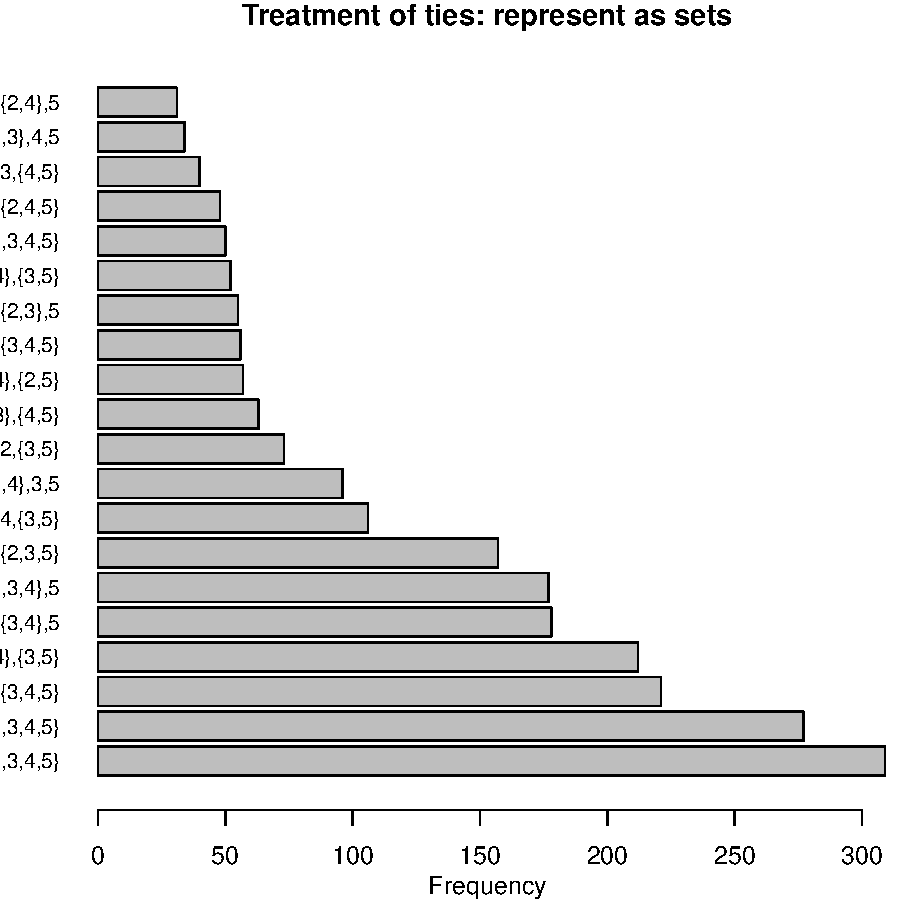
\includegraphics{anchors-vignette-order}

Details of how to interpret and use the output of the summary are
provided in \cite{wand.ea:2007}, where it is discussed in detail how
\code{vign6} is given the highest response almost half the
time, however \code{vign4} is more often given the highest response
than \code{vign5}.  

In light of this it is worth reestimating $C$ using the consensus
ordering of the vignettes,
\begin{Schunk}
\begin{Sinput}
> a2 <- anchors(self ~ vign2+vign3+vign5+vign4+vign6, freedom, method="C")
> summary(a2)
\end{Sinput}
\begin{Soutput}
ANCHORS: SUMMARY OF RELATIVE RANK ANALYSIS:

Overview of C-ranks

Number of cases: 1654 with interval value, 1846 with scalar value

Maximum possible C-rank value: 11

Interval on C-scale: Frequency and proportions Cs to Ce
           N  Prop MinEnt
 1 to  1 387 0.111      1
 2 to  2 279 0.080      2
 3 to  3 336 0.096      3
 4 to  4  81 0.023      4
 5 to  5  59 0.017      5
 6 to  6  80 0.023      6
 7 to  7  38 0.011      7
 8 to  8  61 0.017      8
 9 to  9  22 0.006      9
10 to 10 164 0.047     10
11 to 11 339 0.097     11
 1 to  4  16 0.005      1
 1 to  5  12 0.003      1
 1 to  6  20 0.006      6
 1 to  7   1 0.000      6
 1 to  8  39 0.011      6
 1 to  9   6 0.002      6
 1 to 10  32 0.009      6
 1 to 11  19 0.005      6
 2 to  4  15 0.004      3
 2 to  5  11 0.003      3
 2 to  6  31 0.009      6
 2 to  7   6 0.002      6
 2 to  8  51 0.015      6
 2 to  9   8 0.002      6
 2 to 10 177 0.051      6
 2 to 11  91 0.026      6
 3 to  6  63 0.018      6
 3 to  7  19 0.005      6
 3 to  8  67 0.019      6
 3 to  9   7 0.002      6
 3 to 10  16 0.005      6
 3 to 11  11 0.003      6
 4 to  6  59 0.017      6
 4 to  7  17 0.005      6
 4 to  8  60 0.017      6
 4 to  9  15 0.004      6
 4 to 10 175 0.050      6
 4 to 11  39 0.011      6
 5 to  8  28 0.008      6
 5 to  9  11 0.003      6
 5 to 10   9 0.003      6
 5 to 11   6 0.002      6
 6 to  8 107 0.031      6
 6 to  9  31 0.009      6
 6 to 10 158 0.045      6
 6 to 11  50 0.014      6
 7 to 10   3 0.001     10
 7 to 11   1 0.000     11
 8 to 10 126 0.036     10
 8 to 11  41 0.012     11

Note: MinEnt is the rank for the interval that minimizes entropy

Summary of C-ranks with ties/intervals broken:

Distribution of ranks omiting interval cases
    1     2     3     4     5     6     7     8     9    10
 0.21 0.151 0.182 0.044 0.032 0.043 0.021 0.033 0.012 0.089
    11
 0.184

Distribution of ranks allocating interval cases uniformly
     1   2     3     4     5     6     7    8     9    10
 0.116 0.1 0.127 0.073 0.068 0.096 0.072 0.09 0.057 0.093
    11
 0.107

Distribution of ranks allocating interval cases via cpolr
and conditioning on observed ranks
    1     2     3     4     5     6     7     8     9    10 
0.118 0.103 0.144 0.056 0.042 0.147 0.037 0.120 0.016 0.107 
   11 
0.110 

Allocating cases to their MinEnt values produces
    1     2     3     4     5     6     7     8     9    10 
0.119 0.080 0.103 0.023 0.017 0.431 0.011 0.017 0.006 0.084 
   11 
0.109 
\end{Soutput}
\end{Schunk}
Changing the assumed ordering of the vignettes increased the number of
cases without any order violation by 60 percent.  With respect to the
top sets of types of ordering,

The analysis of vignettes is useful both at the stage of evaluating a
pilot study of survey instruments, as well at the stage of choosing
how (and whether) to use particular vignettes.  The results of
non-parametric anchoring vignettes analysis using $C$ are entirely
dependent on which vignettes are included and the order in which they
are specified.
% For further discussion on diagnosing problems in
% vignettes see \cite{wand:2007}.

\subsection{Example Code: \texttt{Subsets of vignettes}}

Calculating entropy for subsets of vignettes as suggested by Wand and
King (2007) is straightforward.  The \code{anchors(...,combn=TRUE)}
calculates statistics of interest, including entropy measures, for
every ordered combination of vignettes.  For more details, please see {\tt
help(anchors.combn)} in R and \cite{king.wand:2007}.
\begin{Schunk}
\begin{Sinput}
> data(freedom)
> fo <- list(self = self ~ 1,
+            vign = cbind(vign1,vign3,vign6) ~ 1, 
+            cpolr= ~ as.factor(country) + sex + age + educ)
> ent <- anchors(fo, data = freedom, method="C", combn=TRUE)
\end{Sinput}
\end{Schunk}
\begin{Schunk}
\begin{Sinput}
> summary(ent,digits=3)
\end{Sinput}
\begin{Soutput}
ANCHORS: SUMMARY OF RELATIVE RANK ANALYSIS:

Overview of C-ranks

Number of cases: 522 with interval value, 2925 with scalar value

Maximum possible C-rank value: 7

Interval on C-scale: Frequency and proportions Cs to Ce
           N  Prop MinEnt
 1 to  1 496 0.144      1
 2 to  2 225 0.065      2
 3 to  3 492 0.143      3
 4 to  4 236 0.068      4
 5 to  5 497 0.144      5
 6 to  6 489 0.142      6
 7 to  7 490 0.142      7
 1 to  4  22 0.006      3
 1 to  5   1 0.000      5
 1 to  6  28 0.008      5
 1 to  7  12 0.003      5
 2 to  4  39 0.011      3
 2 to  5  10 0.003      5
 2 to  6 124 0.036      5
 2 to  7  31 0.009      5
 3 to  6   9 0.003      5
 3 to  7   9 0.003      5
 4 to  6 193 0.056      5
 4 to  7  44 0.013      5

Note: MinEnt is the rank for the interval that minimizes entropy

Summary of C-ranks with ties/intervals broken:

Distribution of ranks omiting interval cases
    1     2     3     4    5     6     7
 0.17 0.077 0.168 0.081 0.17 0.167 0.168

Distribution of ranks allocating interval cases uniformly
     1     2     3     4     5     6     7
 0.147 0.082 0.161 0.108 0.179 0.175 0.148

Distribution of ranks allocating interval cases via cpolr
and conditioning on observed ranks
    1     2     3     4     5     6     7 
0.148 0.075 0.165 0.094 0.187 0.183 0.148 

Allocating cases to their MinEnt values produces
    1     2     3     4     5     6     7 
0.144 0.065 0.160 0.068 0.278 0.142 0.142 

Summary of entropy and intervals by subsets of vignettes:

  Vignettes Estimated entropy Minimum entropy
1       123             1.903           1.844
4        12             1.450           1.430
3        13             1.490           1.465
2        23             1.527           1.489
7         1             0.795           0.795
6         3             0.959           0.959
5         2             1.044           1.044
  Interval Cases Span avg. Max. rank
1            522     1.471         7
4            220     1.151         5
3            195     1.137         5
2            418     1.285         5
7              0     1.000         3
6              0     1.000         3
5              0     1.000         3
\end{Soutput}
\end{Schunk}
One important feature to be noted about including
\code{cpolr=} variables is that cases with any missing value in the
covariates will be listwise deleted for both both the estimated and
minimum entropy calculations to ensure a common basis for comparisons.
As such, the minimum entropy values may change as a function of what
variables (if any) are included in \code{cpolr=}.

The {\tt plot()} method is described in
\code{help(plot.anchors.rank)}, and an example is given here,
\begin{Schunk}
\begin{Sinput}
> plot(ent)
\end{Sinput}
\end{Schunk}
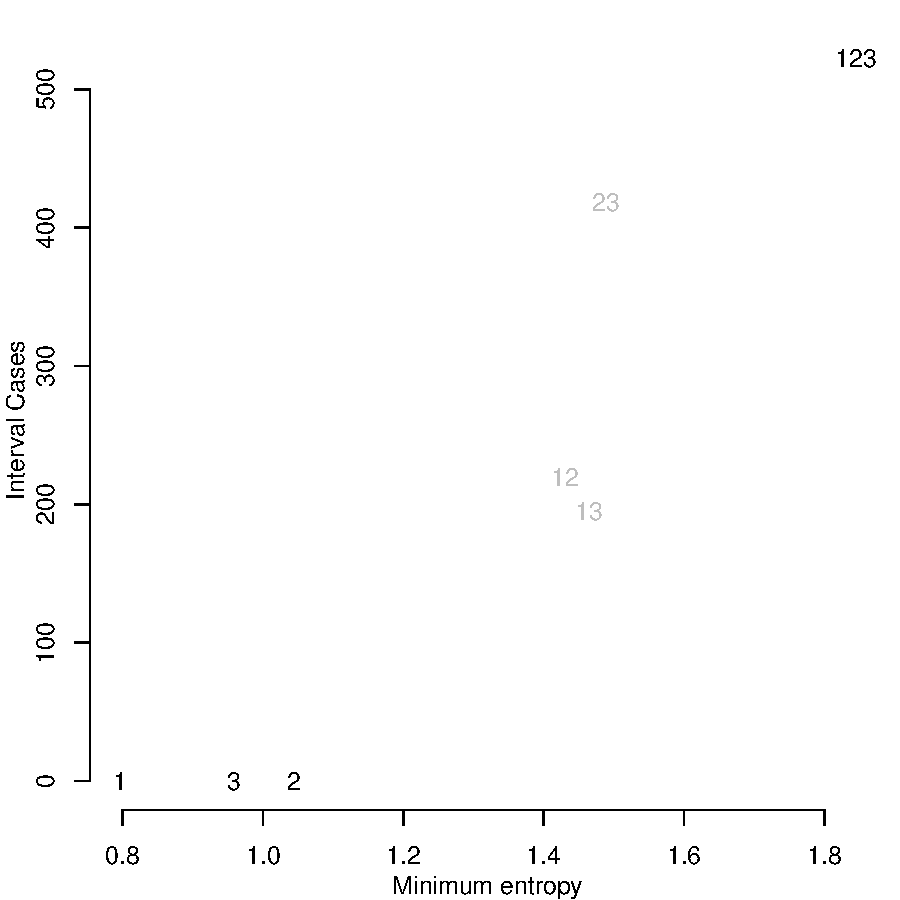
\includegraphics{anchors-entropy1}
% <<results = hide,label=entropy2,fig=TRUE>>=
% plot(ent,xy=c("minimum","interval")
% @ 

\section{Parametric Model}

\noindent
This section describes the Compound Hierarchical Ordered Probit
(chopit) model.

\subsection{Self-assessment component}

Figure \ref{f:self} summarizes the self-assessment component of the
model.
\begin{figure}[t]
  \begin{center}
    \xymatrix@C=13pt{ &
      % & & & &
      & & & X_i \ar[dr]^{\beta}& & {\eta_i}\ar[dl] &
      \omega^2\ar@{~>}[l]
      \\
%%%
%%%
      \text{Actual:} &
      % &{\theta_1}\ar[d] &{\cdots} &{\theta_J}\ar[d] &
      & &&&{\mu_i}\ar[dll]\ar[d]\ar[drr]
      \\
%%%
%%%
      \text{Perceived:} &
      % {\sigma^2}\ar@{~>}[r] &{Z_{\ell
      %     1}^*}\ar[d]_{V_{\ell}\xrightarrow{\gamma_1}\tau_{\ell 1}}
      % &{\cdots} &{Z_{\ell J}^*}\ar[d]^{\tau_{\ell
      %     1}\xleftarrow{\Cr{\gamma_1}}V_{\ell}} &
      % {\sigma^2}\ar@{~>}[l]
      & \sigma_1^2\ar@{~>}[r] &
      {Y_{i1}^*}\ar[d]_{V_i\xrightarrow{\gamma_1}\tau_{i1}} &
      \sigma^2_2\ar@{~>}[r] &
      {Y_{i2}^*}\ar[d]_{V_i\xrightarrow{\gamma_2}\tau_{i2}} &{\cdots}
      & {Y_{iS}^*}\ar[d]^{\tau_{iS}\xleftarrow{\gamma_S}V_i} &
      \sigma^2_S\ar@{~>}[l]
      \\
%%%
%%%
      \text{Reported:} &
      % &{z_{\ell 1}} &{\cdots } &{z_{\ell J} }&
%
      &&{y_{i1}} &&{y_{i2}} &{\cdots } &{y_{iS}}
      \\
    }
    \caption{\label{f:self}Self-Assessment Component: All levels vary
      over observations $i$.  Each solid arrow denotes a deterministic
      effect; a squiggly arrow denotes the addition of normal random
      error with variance indicated at the arrow's source.}
  \end{center}
\end{figure}

The \emph{actual} level for respondent $i$ is $\mu_i$, a continuous
unidimensional variable (with higher values indicating more freedom,
better health, etc., defined by the order of the vignettes).
Respondent $i$ perceives $\mu_i$ only with random normal error so that
\begin{equation}
  \label{stoch-s}
  Y_{is}^* \sim N(\mu_i,\sigma^2_s)
\end{equation}
is respondent $i$'s unobserved \emph{perceived} level.  The actual
level is a linear function of observed covariates $X_i$, the first
column of which can be a constant term (if it is not needed for
identification) and an independent normal random effect $\eta_i$:
\begin{equation}
  \label{syst-s}
  \mu_i = X_i\beta + \eta_i
\end{equation}
with parameter $\beta$ and
\begin{equation}
  \label{re}
  \eta_i \sim N(0,\omega^2).
\end{equation}

The \emph{reported} survey response category is $y_{is}$ and is
generated by the model via this observation mechanism:
\begin{equation}
  \label{obsmech-s}
  y_{is} = k \qquad \text{if $\tau_{is}^{k-1}\leq Y_{is}^* < \tau_{is}^k$}
\end{equation}
with a vector of thresholds $\tau_{is}$ (where $\tau_{is}^0=-\infty$,
$\tau_{is}^{K_s}=\infty$, and $\tau^{k-1}_{is}<\tau^k_{is}$, with
indexes for categories $k=1,\dots,K_s$ and self-assessment questions
$s=1,\dots,S$) that vary over the observations as a function of a
vector of covariates, $V_i$ (the first column of which can be a
constant term), and unknown parameter vectors $\gamma_s$ (with
elements the vector $\gamma_s^k$):
\begin{align}
  \label{taus}
  \tau_{is}^1 &= \gamma_s^1 V_i \\ \notag \tau_{is}^k &=
  \tau^{k-1}_{is}+e^{\gamma_s^k V_i}\qquad (k=2,\dots,K_s-1)
\end{align}

\subsection{Vignette Component}

Figure \ref{f:vign} summarizes the vignette component of the model for
question set $s$ ($s=1,\dots,S$).  Under the model, one or more of the
self-assessment questions have corresponding vignettes.
\begin{figure}[t]
  \begin{center}
    \xymatrix@C=13pt{ &
      % & & & & & & & X_i \ar[dr]^{\beta}& & {\eta_i}\ar[dl] &
      % \omega^2\ar@{~>}[l]
      \\
%%%
%%%
      \text{Actual:} & &{\theta_1}\ar[d] &{\cdots}
      &{\theta_{J_s}}\ar[d] &
      % & &&&\Cb{{\mu_i}}\ar[dll]\ar[d]\ar[drr]
      \\
%%%
%%%
      \text{Perceived:} & {\sigma^2_{s1}}\ar@{~>}[r] &{Z_{\ell
          s1}^*}\ar[d]_{V_{\ell}\xrightarrow{\gamma_s}\tau_{\ell s}}
      &{\cdots} &{Z_{\ell s{J_s}}^*}\ar[d]^{\tau_{\ell
          s}\xleftarrow{\gamma_s}V_{\ell}} &
      {\sigma^2_{s{J_s}}}\ar@{~>}[l]
      % & 1\ar@{~>}[r] &
      % {Y_{i1}^*}\ar[d]_{V_i\xrightarrow{\Cr{\gamma_1}}\tau_{i1}} &
      % 1\ar@{~>}[r] &
      % {Y_{i2}^*}\ar[d]_{V_i\xrightarrow{\gamma_2}\tau_{i2}}
      % &{\cdots} &
      % {Y_{iS}^*}\ar[d]^{\tau_{iS}\xleftarrow{\gamma_S}V_i} &
      % 1\ar@{~>}[l]
      \\
%%%
%%%
      \text{Reported:} & &{z_{\ell s1}} &{\cdots } &{z_{\ell s{J_s}}
      }&
      % &&{y_{i1}} &&{y_{i2}} &{\cdots } &{y_{iS}}
      \\
    }
  \end{center}
  \caption{\label{f:vign}Vignette Component for question set $s$
    ($s=1,\dots,S'$, $S'\leq S$).  All levels vary over observations
    $\ell$.  Each solid arrow denotes a deterministic effect; a
    squiggly arrow denotes the addition of normal random error with
    variance indicated at the arrow's source.}
\end{figure}

The actual level for vignette $j$ is $\theta_j$ ($j=1,\dots,J_s$),
measured on the same scale as $\mu_i$ and the $\tau$'s.  Respondent
$\ell$ perceives $\theta_j$ with random normal error so that
\begin{equation}
  \label{stoch-v}
  Z_{{\ell}sj}^* \sim N(\theta_j,\sigma^2_{sj})
\end{equation}
represents respondent ${\ell}$'s unobserved assessment of the level of
vignette $j$ for question set $s$.

The perception of respondent ${\ell}$ about the level of vignette $j$
elicited via a survey question $s$ with the same $K_s$ ordinal
categories as the corresponding self-assessment question.  Thus, the
respondent turns the continuous $Z_{{\ell}sj}^*$ into a categorical
answer to the survey question $z_{{\ell}sj}$ via this observation
mechanism:
\begin{equation}
  \label{obsmech-v}
  z_{{\ell}sj} = k \qquad \text{if $\tau_{\ell s}^{k-1}\leq Z_{{\ell}j}^* 
    < \tau_{\ell s}^k$}
\end{equation}
with thresholds determined by the same $\gamma_s$ coefficients as in
(\ref{taus}) for $y_{i1}$, and the same explanatory variables but with
values measured for units $\ell$, $V_{\ell}$:
\begin{align}
  \label{taus-v}
  \tau_{{\ell}1}^1 &= \gamma_s^1 V_{\ell} \\ \notag \tau_{{\ell}1}^k
  &= \tau^{k-1}_{{\ell}s} +e^{\gamma_s^k V_{\ell}}\qquad
  (k=2,\dots,K_1-1).
\end{align}

\subsection{Identification}

The model as specified above has an infinite number of equivalent
maximum likelihood solutions.  To identify the model, two choices must
be made:
\begin{enumerate}
\item The mean of the actual level must be set, by choosing one point.
  This can be done by setting the constant term $\beta_0=0$ (in which
  case be aware of your choice of the scale of the variables in $X$),
  or one of the $\theta$'s.
\item The variance of the actual level must also be set.  This can be
  done by setting all the self-assessment variances (such as
  $\sigma^2_s=1$, for all $s$) or by setting another point among
  $\beta_0$ or the $\theta$'s.
\end{enumerate}
Two common parameterizations are as follows:
\begin{enumerate}
\item The ordinal probit parameterization is useful for comparing
  chopit to this simpler model.  Set $\beta_0=0$ and
  $\sigma^2_1=\dots=\sigma^2_S=1$.
\item Another option is parameterization defined by the extreme
  vignettes.  Let $\theta_1=0$ and $\theta_{J_s}=1$.  This lets
  estimates of $\mu$ be interpreted on the scale of the vignettes,
  with 0 being the level of the lowest vignette and 1 the level of the
  highest.  Note that $\mu$ can still be higher than 1 or lower than 0,
  but the units are easily interpretable.
\end{enumerate}

\ssubsection{Example Code}{chopit()}

The \code{chopit()} function provided by \pkg{anchors} at it's most
basic simply requires specifying the formula's defining $y$s, $z$s,
and $\tau$s.  For example, using variables from the
\code{data(freedom)} dataset, we have the {\em named} list.
\begin{Schunk}
\begin{Sinput}
> fo <- list(self =  self ~ sex + age + educ + factor(country) ,
+              vign = cbind(vign1,vign2,vign3,vign4,vign5,vign6) ~ 1 ,
+              tau  =       ~ sex + age + educ + factor(country) )
\end{Sinput}
\end{Schunk}
The names \code{self=}, \code{vign=}, and \code{tau=} as written, are
required.  On the LHS of the equality signs are the variables of the
dataset that specify the details of the models as for other models
(e.g., \code{lm()}).

The self-assessment variable \code{self} is modeled to have a mean
that is a linear additive function of \code{sex}, \code{age},
\code{educ} and \code{country} dummies.  The vignettes are specified
as a vector of outcomes
\code{cbind(vign1,vign2,vign3,vign4,vign5,vign6)} as a function of
only an intercept '\code{$\sim$ 1}'.  This is both a simple and
accurate way to describe the model of $\theta$s which are the mean
locations of the vignettes.  The $\tau$ cutpoints shared by the
self-assessment and the vignettes are specified as their own formula
without a LHS variable.

Beyond the formula and data, the rest will be set by default in the
basic invocation,
\begin{Schunk}
\begin{Sinput}
> out  <- chopit( fo, data=freedom)
\end{Sinput}
\end{Schunk}
which can be summarized by the \code{summary} method,
\begin{Schunk}
\begin{Sinput}
> summary(out)
\end{Sinput}
\begin{Soutput}
ANCHORS: SUMMARY OF RELATIVE CHOPIT ANALYSIS:

Model formula:
$self
self ~ sex + age + educ + factor(country)

$vign
cbind(vign1, vign2, vign3, vign4, vign5, vign6) ~ 1

$tau
~sex + age + educ + factor(country)

$cpolr
~1
<environment: 0x7fb3efed0340>


Coefficients:
                                    coeff     se
gamma.cut1.(Intercept)            -1.6697 0.0774
gamma.cut1.sex                     0.0570 0.0228
gamma.cut1.age                    -0.0028 0.0007
gamma.cut1.educ                    0.0109 0.0068
gamma.cut1.factor(country)Eurasia  0.0447 0.0504
gamma.cut1.factor(country)Oceania -0.1262 0.0309
gamma.cut2.(Intercept)             0.6655 0.0388
gamma.cut2.sex                    -0.0426 0.0205
gamma.cut2.age                     0.0013 0.0006
gamma.cut2.educ                   -0.0140 0.0061
gamma.cut2.factor(country)Eurasia -0.0286 0.0449
gamma.cut2.factor(country)Oceania  0.0260 0.0274
gamma.cut3.(Intercept)             0.7068 0.0319
gamma.cut3.sex                    -0.0211 0.0167
gamma.cut3.age                    -0.0001 0.0005
gamma.cut3.educ                    0.0112 0.0051
gamma.cut3.factor(country)Eurasia  0.0250 0.0374
gamma.cut3.factor(country)Oceania -0.0985 0.0218
gamma.cut4.(Intercept)             0.5937 0.0294
gamma.cut4.sex                     0.0436 0.0159
gamma.cut4.age                     0.0007 0.0005
gamma.cut4.educ                    0.0163 0.0049
gamma.cut4.factor(country)Eurasia  0.0605 0.0365
gamma.cut4.factor(country)Oceania  0.0166 0.0211
sigma.random.effect                1.0000    NaN
sigma.self                         1.0000    NaN
sigma.vign1                        0.7951 0.0183
sigma.vign2                        0.9974 0.0239
sigma.vign3                        0.7546 0.0173
sigma.vign4                        0.8336 0.0208
sigma.vign5                        0.7246 0.0171
sigma.vign6                        1.3307 0.0420
theta.vign1                       -1.0863 0.0721
theta.vign2                       -1.2051 0.0734
theta.vign3                       -0.2478 0.0706
theta.vign4                        0.1660 0.0715
theta.vign5                       -0.0562 0.0706
theta.vign6                        0.9519 0.0820
beta.(Intercept)                   0.0000    NaN
beta.sex                           0.1434 0.0388
beta.age                          -0.0019 0.0012
beta.educ                         -0.0569 0.0117
beta.factor(country)Eurasia        0.4600 0.0897
beta.factor(country)Oceania       -0.7019 0.0517

-Log-likelihood of CHOPIT:  32421.69 

Partition of CHOPIT -Log-likelihood by question:
                 -LL    N
Self (self) 5154.965 3447
vign1       5032.314 3447
vign2       5207.052 3447
vign3       4766.234 3447
vign4       4340.710 3447
vign5       4485.543 3447
vign6       3434.877 3447

Number of cases that contribute at least partially to likelihoods:
   a) in self-responses: 3447 
   b) in vign-responses: 3447 
\end{Soutput}
\end{Schunk}

The default invocation uses the the ordinal probit normalization,
which identifies/normalizes the model by omitting the intercept in
$\mu$, and setting $\sigma_1=1$ (the variance of the first
self-assessment question).  If one specified the explanatory variables
of \code{self=} to include an intercept, then that intercept parameter
would be constrained to be zero as will be \code{beta.(Intercept)} in
this example.




% \section{List of Datasets} 
% 
% Datasets that can be loaded via \code{data()} are,
% 
% \begin{tabular}{ll}
% chopitsim  & Simulated Data for test chopit function\\
% mexchn     & China-Mexico political efficacy data \\
% poleff     & Simulated Political Efficacy Data \\
% poleffna   & Simulated Political Efficacy Data with NA (demo only, don't use)\\
% freedom    & Individual freedom of speech data\\
% sleep      & Sleep data for china\\
% selfcare   & Self-care data for china\\
% table1     & Reference from Table 1 of King and Wand (2007)\\
% table1src  & Specific response values that have inequalities to create table1\\
% \end{tabular}

\section{List of functions}

Here is a list of function available in \Ranchors, and help
files are available for each of them.
\begin{tabular}{ll}
allequal.test           & all.equal with expected outcome test               \\
anchors                 & Analysis of surveys with anchoring vignettes       \\
anchors.chopit          & Compound Hierarchical Ordered Probit (CHOPIT)	     \\
anchors.combn           & Calculate known minimum or estimated entropy for subsets\\
anchors.data            & Organized data from surveys with anchoring	     \\
anchors.options         & Set or query anchors() parameters		     \\
anchors.order           & Calculate frequency of vignette orderings	     \\
anchors.rank            & Non-parametric analysis of surveys with	     \\
convert                 & Convert factor variables into integers	     \\
cpolr                   & Censored ordered probit			     \\
fitted.anchors.cpolr    & Conditional and unconditional prediction for cpolr \\
fitted.anchors.rank     & Fitted values of non-parametric models	     \\
fitted.cpolr            & Conditional and unconditional prediction for cpolr \\
insert                  & Insert DIF-corrected variable into dataframe	     \\
barplot.anchors.order   & Plot frequency of vignette orderings		     \\
barplot.anchors.rank    & Plot distribution of non-parametric ranks	     \\
replace.list            & Updating contents of one list using a second	     \\
replace.value           & Replaces occurences of a value with another	     \\
summary.anchors.chopit  & Summary of CHOPIT Analysis			     \\
summary.anchors.order   & Calculate frequency of vignette orderings	     \\
summary.anchors.rank    & Summary of non-parameteric anchors analysis	     \\
trim.data               & Trim a dataset to match anchors.data               \\   
\end{tabular}


% \section{List of Replication files} 
% 
% As an aid to those who would simply like to re-compute published
% results that use this or earlier versions of this package, we include
% this list.  
% 
% \begin{tabular}{ll}
% chopit.mexchn   &   King et al (2004) Table 2 (non-linear taus)\\
% anchors.freedom3&   Wand et al (2007) Figure 2 histogram with 3 vignettes  \\
% anchors.freedom6&   Wand et al (2007) Figure 1 histogram with 6 vignettes  \\
% anchors.mexchn  &   King and Wand (2007) Figure 1 histogram   \\
% entropy.mexchn  &   King and Wand (2007) Figure 2 entropy()   \\
% entropy.sleep   &   King and Wand (2007) Figure 3 entropy()   \\
% entropy.self    &   King and Wand (2007) Figure 4 entropy()   \\
% anchors.vign2   &   King and Wand (2007) Table 1 anchors()   \\
% \end{tabular}
% 
% Any of these can be invoked with \code{demo()}, for example,
% <<eval=FALSE>>=
% demo(anchors)
% @ 
% 
% Additional demo files include,
% 
% \begin{tabular}{ll}
% anchors		&  Demo of anchors: summary, plot     \\
% chopit 		&  Demo of chopit: summary, plot      \\
% chopit.re       &  Demo of chopit: with random effects\\
% \end{tabular}
% 
% which can be invoked in the same manner with \code{demo()}.
\newpage
\bibliographystyle{apsr2001}
\bibliography{anchors}
\end{document}


%%% Local Variables: 
%%% mode: latex
%%% TeX-master: "anchors.Rnw"
%%% End: 
% LocalWords:  eval Sweavehook mpg
% LocalWords:  probit chopit cpolr polr vign
% LocalWords:  combinatoric covariates
% LocalWords:  dataset datasets
% LocalWords:  mexchn poleff poleffna
% LocalWords:  LocalWords 
